%
%===============>>  ГРУППА 9-2 МОДУЛЬ 8  <<=============
%
\setmodule{8}

%BEGIN_FOLD % ====>>_____ Занятие 1 _____<<====
\begin{class}[number=1]
	\begin{listofex}
		\item Первый сплав содержит \( 5\% \) меди, второй --- \( 11\% \) меди. Масса второго сплава больше массы первого на \( 4 \) кг. Из этих двух сплавов получили третий сплав, содержащий \( 10\% \) меди. Найдите массу третьего сплава.
		\item Смешали некоторое количество \( 19 \)-процентного раствора некоторого вещества с таким же количеством \( 23 \)-процентного раствора этого же вещества. Сколько процентов составляет концентрация получившегося раствора?
		\item Смешали некоторое количество \( 82 \)-процентного раствора некоторого вещества с таким же количеством \( 94 \)-процентного раствора этого же вещества. Сколько процентов составляет концентрация получившегося раствора?
		\item Имеются два сосуда, содержащие \( 24 \) кг и \( 26 \) кг раствора кислоты различной концентрации. Если их слить вместе, то получится раствор, содержащий \( 39\% \) кислоты. Если же слить равные массы этих растворов, то полученный раствор будет содержать \( 40\% \) кислоты. Сколько килограммов кислоты содержится в первом растворе?
		\item Имеются два сосуда, содержащие \( 30 \) кг и \( 42 \) кг раствора кислоты различной концентрации. Если их слить вместе, то получим раствор, содержащий \( 40\% \) кислоты. Если же слить равные массы этих растворов, то полученный раствор будет содержать \( 37\% \) кислоты. Сколько килограммов кислоты содержится во втором растворе?
		\item Свежие фрукты содержат \( 93\% \) воды, а высушенные --- \( 16\% \). Сколько сухих фруктов получится из \( 252 \) кг свежих фруктов?
		\item Имеется два сплава с разным содержанием меди: в первом содержится \( 60\% \), а во втором --- \( 45\% \) меди. В каком отношении надо взять первый и второй сплавы, чтобы получить из них новый сплав, содержащий \( 55\% \) меди?
		\item При смешивании первого раствора кислоты, концентрация которого \( 30\% \), и второго раствора этой же кислоты, концентрация которого \( 50\% \), получили раствор, содержащий \( 45\% \) кислоты. В каком отношении были взяты первый и второй растворы?
		\item Решите уравнение: \((x-2)(x-3)(x-5)=(x-3)(x-4)(x-5)\)
	\end{listofex}
\end{class}
%END_FOLD

%BEGIN_FOLD % ====>>_____ Занятие 2 _____<<====
\begin{class}[number=2]
	\begin{listofex}
		\item Свежие фрукты содержат \( 75\% \) воды, а высушенные --- \( 25\% \). Сколько сухих фруктов получится из \( 135 \) кг свежих фруктов?
		\item Смешали некоторое количество \( 82 \)-процентного раствора некоторого вещества с таким же количеством \( 94 \)-процентного раствора этого же вещества. Сколько процентов составляет концентрация получившегося раствора?
		\item Дима и Саша выполняют одинаковый тест. Дима отвечает за час на \( 12 \) вопросов теста, а Саша --- на \( 22 \). Они одновременно начали отвечать на вопросы теста, и Дима закончил свой тест позже Саши на \( 75 \) минут. Сколько вопросов содержит тест?
		\item Игорь и Паша красят забор за \( 18 \) часов. Паша и Володя красят этот же забор за \( 20 \) часов, а Володя и Игорь --- за \( 30 \) часов. За сколько минут мальчики покрасят забор, работая втроём?
		\item Первый рабочий за час делает на \( 10 \) деталей больше, чем второй, и выполняет заказ, состоящий из \( 60 \) деталей, на \( 3 \) часа быстрее, чем второй рабочий, выполняющий такой же заказ. Сколько деталей в час делает второй рабочий?
		\item На изготовление \( 231 \) детали ученик тратит на \( 11 \) часов больше, чем мастер на изготовление \( 462 \) таких же деталей. Известно, что ученик за час делает на \( 4 \) детали меньше, чем мастер. Сколько деталей в час делает ученик?
		\item Три бригады изготовили вместе \( 248 \) деталей. Известно, что вторая бригада изготовила деталей в \( 4 \) раза больше, чем первая и на \( 5 \) деталей меньше, чем третья. На сколько деталей больше изготовила третья бригада, чем первая?
		\item Две трубы наполняют бассейн за \( 6 \) часов \( 18 \) минут, а одна первая труба наполняет бассейн за \( 9 \) часов. За сколько часов наполняет бассейн одна вторая труба?
		\item Чтобы накачать в бак \( 117 \) л воды, требуется на \( 5 \) минут больше времени, чем на то, чтобы выкачать из него \( 96 \) л воды. За одну минуту можно выкачать на \( 3 \) л воды больше, чем накачать. Сколько литров воды накачивается в бак за минуту?
		\item Первая труба пропускает на \( 2 \) литра воды в минуту меньше, чем вторая. Сколько литров воды в минуту пропускает вторая труба, если резервуар объёмом \( 130 \) литров она заполняет на \( 4 \) минуты быстрее, чем первая труба заполняет резервуар объёмом \( 136 \) литров?
		\item Решите уравнения:
		\begin{tasks}(2)
			\task \( (x^2+x-1)(x^2+x+2)=40 \)
			\task \( (2x^2+x-1)(2x^2+x-4)+2=0 \)
		\end{tasks}
	\end{listofex}
\end{class}
%END_FOLD

%BEGIN_FOLD % ====>>_ Домашняя работа 1 _<<====
\begin{homework}[number=1]
	\begin{listofex}\item Сократите дроби:
		\begin{tasks}(2)
			\task \( \dfrac{(2a^2)^3\cdot(3b)^2}{(6a^3b)^2} \)
			\task \( \dfrac{(3x)^3\cdot x^{-9}}{x^{-10}\cdot2x^4} \)
		\end{tasks}
		\item При смешивании первого раствора кислоты, концентрация которого \( 40\% \), и второго раствора этой же кислоты, концентрация которого \( 48\% \), получили раствор, содержащий \( 42\% \) кислоты. В каком отношении были взяты первый и второй растворы?
		Имеется два сплава с разным содержанием золота: в первом содержится \( 50\% \), а во втором --- \( 80\% \) золота. В каком отношении надо взять первый и второй сплавы, чтобы получить из них новый сплав, содержащий \( 55\% \) золота?
		\item Дима и Саша выполняют одинаковый тест. Дима отвечает за час на \( 19 \) вопросов теста, а Саша --- на \( 20 \). Они одновременно начали отвечать на вопросы теста, и Дима закончил свой тест позже Саши на \( 9 \) минут. Сколько вопросов содержит тест?
		\item Две трубы наполняют бассейн за \( 8 \) часов \( 45 \) минут, а одна первая труба наполняет бассейн за \( 21 \) часов. За сколько часов наполняет бассейн одна вторая труба?
	\end{listofex}
\end{homework}
%END_FOLD

%BEGIN_FOLD % ====>>_____ Занятие 3 _____<<====
\begin{class}[number=3]
	\begin{listofex}
		\item В выпуклом четырехугольнике \( ABCD \) \( AB=BC \), \( AD=CD \), \( \angle B=60\degree \), \( \angle D=110\degree \). Найдите \( \angle A \). Ответ дайте в градусах.
		\item Углы выпуклого четырехугольника относятся как \( 1:2:3:4 \). Найдите меньший угол. Ответ дайте в градусах.
		\item Два угла вписанного в окружность четырехугольника равны \( 82\degree \) и \( 58\degree \). Найдите больший из оставшихся углов. Ответ дайте в градусах.
		\item Четырёхугольник \( ABCD \) вписан в окружность. Угол \( ABC \) равен \( 136\degree \), угол \( CAD \) равен \( 82\degree \). Найдите угол \( ABD \). Ответ дайте в градусах.
		\item Четырехугольник \( ABCD \) вписан в окружность. Угол \( ABC \) равен \( 70\degree \), угол \( CAD \) равен \( 49\degree \). Найдите угол \( ABD \). Ответ дайте в градусах.
		\item На стороне \( BC \) прямоугольника \( ABCD \), у которого \( AB=12 \) и \( AD=17 \), отмечена точка \( E \) так, что \( \angle EAB=45\degree \). Найдите \( ED \).
		\item Моторная лодка прошла \( 36 \) км по течению реки и вернулась обратно, потратив на весь путь \( 5 \) часов. Скорость течения реки равна \( 3 \) км/ч. Найдите скорость лодки в неподвижной воде.
		\item Баржа прошла по течению реки \( 48 \) км и, повернув обратно, прошла ещё \( 36 \) км, затратив на весь путь \( 6 \) часов. Найдите собственную скорость баржи, если скорость течения реки равна \( 5 \) км/ч.
		\item Теплоход проходит по течению реки до пункта назначения \( 280 \) км и после стоянки возвращается в пункт отправления. Найдите скорость теплохода в неподвижной воде, если скорость течения равна \( 4 \) км/ч, стоянка длится \( 15 \) часов, а в пункт отправления теплоход возвращается через \( 39 \) часов после отплытия из него.
		\item Катер прошёл от одной пристани до другой, расстояние между которыми по реке равно \( 48 \) км, сделал стоянку на \( 20 \) мин и вернулся обратно через \( \mfrac{5}{1}{3} \) ч после начала поездки. Найдите скорость течения реки, если известно, что скорость катера в стоячей воде равна \( 20 \) км/ч.
		\item Из пункта \( A \) в пункт \( B \), расположенный ниже по течению реки, отправился плот. Одновременно навстречу ему из пункта \( B \) вышел катер. Встретив плот, катер сразу повернул и поплыл назад. Какую часть пути от \( A \) до \( B \) пройдет плот к моменту возвращения катера в пункт \( B \), если скорость катера в стоячей воде вчетверо больше скорости течения реки?
		\item Расстояние между пристанями \( A \) и \( B \) равно \( 80 \) км. Из \( A \) в \( B \) по течению реки отправился плот, а через \( 2 \) часа вслед за ним отправилась яхта, которая, прибыв в пункт \( B \), тотчас повернула обратно и возвратилась в \( A \). К этому времени плот прошел \( 22 \) км. Найдите скорость яхты в неподвижной воде, если скорость течения реки равна \( 2 \) км/ч. Ответ дайте в км/ч.
		\item Расстояние между пристанями \( A \) и \( B \) равно \( 126 \) км. Из \( A \) в \( B \) по течению реки отправился плот, а через \( 1 \) час вслед за ним отправилась яхта, которая, прибыв в пункт \( B \), тотчас повернула обратно и возвратилась в \( A \). К этому времени плот прошел \( 34  \) км. Найдите скорость яхты в неподвижной воде, если скорость течения реки равна \( 2 \) км/ч. Ответ дайте в км/ч.
		\item Пристани \( A \) и \( B \) расположены на реке, скорость течения которой на этом участке равна \( 3 \) км/ч. Лодка проходит туда и обратно без остановок со средней скоростью \( 8 \) км/ч. Найдите собственную скорость лодки.
	\end{listofex}
\end{class}
%END_FOLD

%BEGIN_FOLD % ====>>_____ Занятие 4 _____<<====
\begin{class}[number=4]
	\begin{listofex}
		\item В треугольнике \( ABC \) \( AB=BC \), а высота \( AH \) делит сторону \( BC \) на отрезки \( BH=64 \) и \( CH=16 \). Найдите \( \cos B \).
		\item В остроугольном треугольнике \( ABC \) высота \( AH \) равна \( 20\sqrt{3} \), а сторона \( AB \) равна \( 40 \). Найдите \( \cos B \).
		\item В треугольнике \( ABC \) проведены медиана \( BM \) и высота \( BH \). Известно, что \( AC=84 \) и \( BC=BM \). Найдите \( AH \).
		\item В треугольнике \( ABC \) проведена биссектриса \( AL \), угол \( ALC \) равен \( 112\degree \), угол \( ABC \) равен \( 106\degree \). Найдите угол \( ACB \). Ответ дайте в градусах.
		\item У треугольника со сторонами \( 16 \) и \( 2 \) проведены высоты к этим сторонам. Высота, проведённая к первой стороне, равна \( 1 \). Чему равна высота, проведённая ко второй стороне?
		\item Медианы треугольника \( ABC \) пересекаются в точке \( M \). Найдите длину медианы, проведённой к стороне \( BC \), если угол \( BAC \) равен \( 47\degree \), угол \( BMC \) равен \( 133\degree \), \( BC=4\sqrt{3} \).
		\item Прямая \( AD \), перпендикулярная медиане \( BM \) треугольника \( ABC \), делит её пополам. Найдите сторону \( AC \), если сторона \( AB \) равна \( 4 \).
		\item Отрезки \( AB \) и \( DC \) лежат на параллельных прямых, а отрезки \( AC \) и \( BD \) пересекаются в точке \( M \). Найдите \( MC \), если \( AB=16 \), \( DC=24 \), \( AC=25 \).
		\item Найдите отношение двух сторон треугольника, если его медиана, выходящая из их общей вершины, образует с этими сторонами углы в \( 30\degree \) и \( 90\degree \).
		\item Высота треугольника разбивает его основание на два отрезка с длинами \( 8 \) и \( 9 \). Найдите длину этой высоты, если известно, что другая высота треугольника делит ее пополам.
		\item Отрезки \( AB \) и \( DC \) лежат на параллельных прямых, а отрезки \( AC \) и \( BD \) пересекаются в точке \( M \). Найдите \( MC \), если \( AB=13 \), \( DC=65 \), \( AC=42 \).
	\end{listofex}
\end{class}
%END_FOLD

%BEGIN_FOLD % ====>>_ Домашняя работа 2 _<<====
\begin{homework}[number=2]
	\begin{listofex}
		\item У треугольника со сторонами \( 15 \) и \( 3 \) проведены высоты к этим сторонам. Высота, проведённая к первой стороне, равна \( 1 \). Чему равна высота, проведённая ко второй стороне?
		\item В треугольнике \( ABC \) проведены медиана \( BM \) и высота \( BH \). Известно, что \( AC=2 \) и \( BC=BM \). Найдите \( AH \).
		\item Медианы треугольника \( ABC \) пересекаются в точке \( M \). Найдите длину медианы, проведённой к стороне \( BC \), если угол \( BAC \) равен \( 26\degree \), угол \( BMC \) равен \( 154\degree \), \( BC=6\sqrt{3} \).
		\item Прямая \( AD \), перпендикулярная медиане \( BM \) треугольника \( ABC \), делит её пополам. Найдите сторону \( AC \), если сторона \( AB \) равна \( 4 \).
		\item Отрезки \( AB \) и \( DC \) лежат на параллельных прямых, а отрезки \( AC \) и \( BD \) пересекаются в точке \( M \). Найдите \( MC \), если \( AB=16 \), \( DC=24 \), \( AC=25 \).
	\end{listofex}
\end{homework}
%END_FOLD

%BEGIN_FOLD % ====>>_____ Занятие 5 _____<<====
\begin{class}[number=5]
	\begin{listofex}
		\item \begin{minipage}[t]{\bodywidth}
			На стороне \( AC \) треугольника \( ABC \) выбраны точки \( D \) и \( E \) так, что углы \( ADB \) и \( BEC \) равны (см. рис.). Оказалось, что отрезки \( AE \) и \( CD \) тоже равны. Докажите, что треугольник \( ABC \) --- равнобедренный.
		\end{minipage}
		\gapwidth
		\begin{minipage}[t]{\picwidth}
			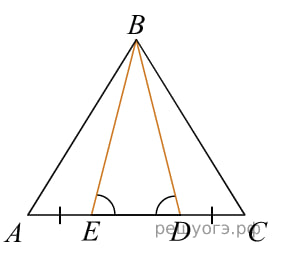
\includegraphics[align=t, width=\linewidth]{\picpath/G91M8C1}
		\end{minipage}
		\item В равностороннем треугольнике \( ABC \) точки \( M \), \( N \), \( K \) --- середины сторон \( AB \), \( BC \), \( CA \) соответственно. Докажите, что треугольник \( MNK \) --- равносторонний.
		\item Докажите, что у равных треугольников \( ABC \) и \( A_1B_1C_1 \) биссектрисы, проведённые из вершины  \( A \) и \( A_1 \), равны.
		\item В треугольнике \( ABC \) угол \( B \) равен \( 36\degree \), \( AB=BC \), \( AD \) --- биссектриса. Докажите, что треугольник \( ABD \) --- равнобедренный.
		\item Докажите, что медиана треугольника делит его на два треугольника, площади которых равны между собой.
		\item Сторона \( BC \) параллелограмма \( ABCD \) вдвое больше стороны \( CD \). Точка \( L \) --- середина стороны \( BC \). Докажите, что \( DL \) --- биссектриса угла \( CDA \).
		\item Докажите, что отрезок, соединяющий середины оснований трапеции, делит её на две равные по площади части.
		\item \begin{minipage}[t]{\bodywidth}
			В параллелограмме \( ABCD \) проведены перпендикуляры \( BE \) и \( DF \) к диагонали \( AC \) (см. рис.). Докажите, что \( BFDE \) --- параллелограмм.
		\end{minipage}
		\gapwidth
		\begin{minipage}[t]{\picwidth}
			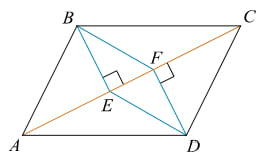
\includegraphics[align=t, width=\linewidth]{\picpath/G92M8L5}
		\end{minipage}
		\item В параллелограмме проведены биссектрисы противоположных углов. Докажите, что отрезки биссектрис, заключенные внутри параллелограмма, равны.
		\item Три стороны параллелограмма равны. Докажите, что отрезок с концами в серединах противоположных сторон параллелограмма равен четверти его периметра.
	\end{listofex}
\end{class}
%END_FOLD

%BEGIN_FOLD % ====>>_____ Занятие 6 _____<<====
\begin{class}[number=6]
	\begin{listofex}
		\item В параллелограмме проведены биссектрисы противоположных углов. Докажите, что отрезки биссектрис, заключенные внутри параллелограмма, равны.
		\item Три стороны параллелограмма равны. Докажите, что отрезок с концами в серединах противоположных сторон параллелограмма равен четверти его периметра.
		\item В окружности через середину \( O \) хорды \( AC \) проведена хорда \( BD \) так, что дуги \( AB \) и \( CD \) равны. Докажите, что \( O \) --- середина хорды \( BD \).
		\item Окружности с центрами в точках \( P \) и \( Q \) не имеют общих точек, и ни одна из них не лежит внутри другой. Внутренняя общая касательная к этим окружностям делит отрезок, соединяющий их центры, в отношении \( a:b \). Докажите, что диаметры этих окружностей относятся как \( a:b \).
		\item В окружности с центром \( O \) проведены две хорды \( AB \) и \( CD \) так, что центральные углы \( AOB \) и \( COD \) равны. На эти хорды опущены перпендикуляры \( OK \) и \( OL \). Докажите, что \( OK \) и \( OL \) равны.
		\item Окружности с центрами в точках \( P \) и \( Q \) пересекаются в точках \( K \) и \( L \), причём точки \( P \) и \( Q \) лежат по одну сторону от прямой \( KL \). Докажите, что прямые \( PQ \) и \( KL \) перпендикулярны.
		\item Окружности с центрами в точках \( I \) и \( J \) пересекаются в точках \( A \) и \( B \), причём точки \( I \) и \( J \) лежат по одну сторону от прямой \( AB \). Докажите, что \( AB\perp IJ \).
	\end{listofex}
\end{class}
%END_FOLD

%BEGIN_FOLD % ====>>_ Домашняя работа 3 _<<====
\begin{homework}[number=3]
	\begin{listofex}
		\item Домашняя работа 3
	\end{listofex}
\end{homework}
%END_FOLD

%BEGIN_FOLD % ====>>_____ Занятие 7 _____<<====
\begin{class}[number=7]
	\title{Подготовка к проверочной}
	\begin{listofex}
		\item Занятие 7
	\end{listofex}
\end{class}
%END_FOLD

=%BEGIN_FOLD % ====>>_ Проверочная работа _<<====
\begin{exam}
	\begin{listofex}
		\item Проверочная
	\end{listofex}
\end{exam}
%END_FOLD